\documentclass[11pt, a4paper]{article}
\usepackage[utf8]{inputenc}
\usepackage{amsmath, amssymb, amsthm}
\usepackage{graphicx}
\usepackage{geometry}
\geometry{a4paper, margin=1in}
\usepackage{hyperref}
\usepackage{float}
\usepackage{booktabs}
\usepackage{listings}
\usepackage{xcolor}
\usepackage{titlesec}
\usepackage{caption}

\titleformat{\section}{\Large\bfseries\sffamily}{\thesection}{1em}{}[\titlerule]
\titleformat{\subsection}{\large\bfseries\sffamily}{\thesubsection}{1em}{}

\definecolor{codegreen}{rgb}{0,0.6,0}
\definecolor{codegray}{rgb}{0.5,0.5,0.5}
\definecolor{codepurple}{rgb}{0.58,0,0.82}
\definecolor{backcolour}{rgb}{0.95,0.95,0.92}

\lstdefinestyle{mystyle}{
    backgroundcolor=\color{backcolour},   
    commentstyle=\color{codegreen},
    keywordstyle=\color{magenta},
    numberstyle=\tiny\color{codegray},
    stringstyle=\color{codepurple},
    basicstyle=\ttfamily\footnotesize,
    breakatwhitespace=false,         
    breaklines=true,                 
    captionpos=b,                    
    keepspaces=true,                 
    numbers=left,                    
    numbersep=5pt,                  
    showspaces=false,                
    showstringspaces=false,
    showtabs=false,                  
    tabsize=2
}
\lstset{style=mystyle}

\title{\textbf{Statistical Solutions Report}\\
\large Modules: Estimation, Confidence Intervals, Bayesian Inference, and Linear Models}
\author{Roll No: 17 \\ Name: Manas Pokley}
\date{\today}

\begin{document}

\maketitle
\tableofcontents
\newpage

\section*{Code Repository Link}
The R scripts used for all numerical problems and simulations in this report are available at:

\begin{center}
\Large\textbf{\url{https://github.com/marksman-20/version_1_assignment}}
\end{center}

\newpage

% =====================================================
% MODULE 1: ESTIMATION
% =====================================================
\section{Module 1: Estimation}

\subsection{Problem 4.33: Comparing Estimators for the Normal Distribution}
\textbf{Solution:}
I ran a simulation in R drawing 100,000 samples of size $n=100$ each from $\mathcal{N}(0,1)$, computing the sample mean and sample median for each. Since the true mean and median are both 0, and both estimators are unbiased, the MSE equals the variance.

Theoretically:
\begin{itemize}
    \item Variance of sample mean: $\sigma^2/n = 1/100 = 0.01$
    \item Asymptotic variance of sample median: $\approx \frac{\pi}{2} \cdot \frac{1}{100} \approx 0.0157$
\end{itemize}

\begin{figure}[H]
    \centering
    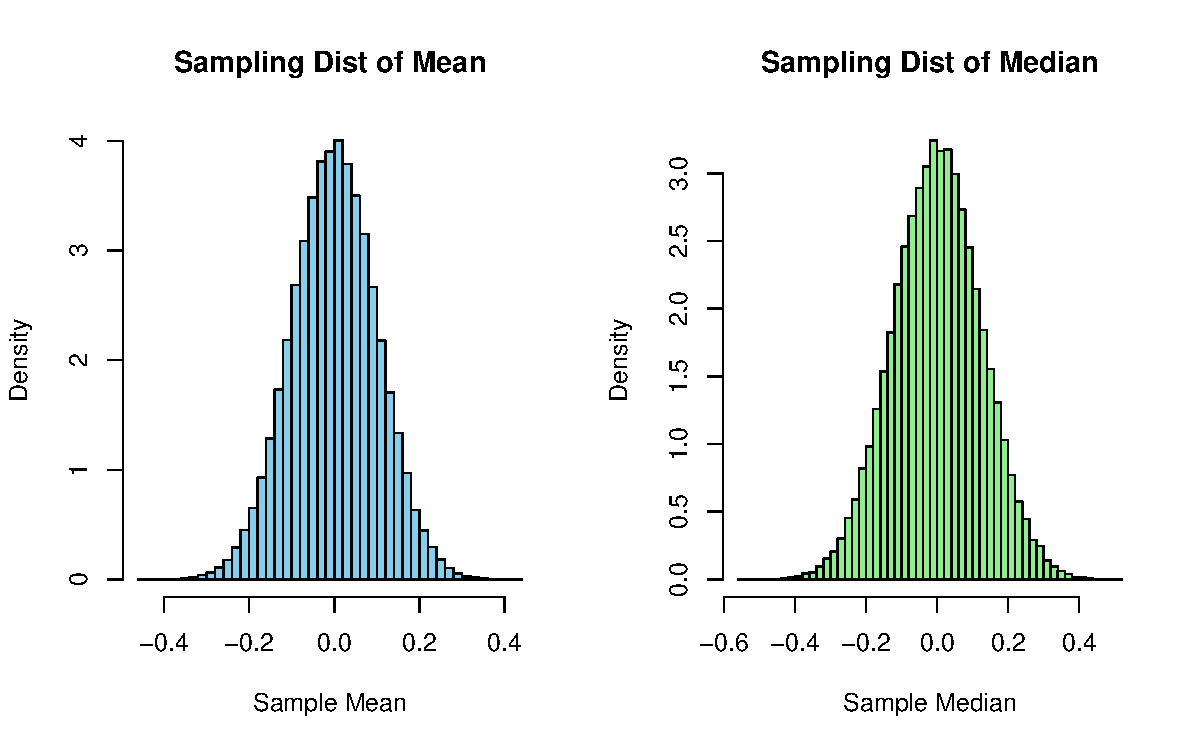
\includegraphics[width=0.8\textwidth]{Estimation_prob1_plot.pdf}
    \caption{Sampling distributions of the sample mean and sample median for $N(0,1)$}
\end{figure}

Simulated MSE from R:
\begin{itemize}
    \item \textbf{MSE of sample mean:} $\approx 0.01004$
    \item \textbf{MSE of sample median:} $\approx 0.01557$
\end{itemize}

The sample mean is the better estimator here. Since it uses all the data equally rather than just the middle values, it is more efficient for a symmetric distribution like the normal.

\subsection{Problem 4.34: Comparing Estimators for the Uniform Distribution}
\textbf{Solution:}
Again using R, I drew 100,000 samples of size $n=100$ from $\mathcal{U}(0,1)$. Both the mean and median of this distribution equal 0.5.

Theory gives:
\begin{itemize}
    \item Variance of sample mean: $\frac{1/12}{100} \approx 0.000833$
    \item Variance of sample median: $\frac{1}{4 \cdot 100 \cdot f(0.5)^2} = \frac{1}{400} = 0.0025$ (since $f(m)=1$ for Uniform)
\end{itemize}

Simulated MSE:
\begin{itemize}
    \item \textbf{MSE of sample mean:} $\approx 0.000833$
    \item \textbf{MSE of sample median:} $\approx 0.002418$
\end{itemize}

The sample mean is again the better estimator — its MSE is about three times smaller. For a uniform distribution there are no extreme outliers to worry about (the distribution is bounded), so the mean's higher sensitivity to all observations works in its favour here.

\newpage
\subsection{Problem 4.36: Bias-Variance Tradeoff for Variance Estimators}
\textbf{Proof:}
Since $\frac{(n-1)S^2}{\sigma^2} \sim \chi^2_{n-1}$, and $\chi^2_k$ has mean $k$ and variance $2k$:
$$E[S^2] = \sigma^2, \quad Var(S^2) = \frac{2\sigma^4}{n-1}$$
So the MSE of the unbiased estimator is:
$$MSE(S^2) = Var(S^2) = \frac{2\sigma^4}{n-1}$$

For the biased estimator $\hat{\sigma}^2 = \frac{n-1}{n} S^2$:
$$E[\hat{\sigma}^2] = \frac{n-1}{n}\sigma^2, \quad \text{Bias} = -\frac{\sigma^2}{n}$$
$$Var(\hat{\sigma}^2) = \frac{(n-1)^2}{n^2} \cdot \frac{2\sigma^4}{n-1} = \frac{2(n-1)\sigma^4}{n^2}$$
$$MSE(\hat{\sigma}^2) = \frac{2(n-1)\sigma^4}{n^2} + \frac{\sigma^4}{n^2} = \frac{2n-1}{n^2}\sigma^4$$

Comparing:
$$\frac{2n-1}{n^2} < \frac{2}{n-1} \iff (2n-1)(n-1) < 2n^2 \iff -3n+1 < 0$$
which holds for all $n \ge 1$. So the biased estimator actually has a lower MSE than the unbiased one — a classic example of how accepting a small bias can reduce variance enough to win overall.

\newpage
\subsection{Problem 4.39: Maximum Likelihood for Exponential Distribution}
\textbf{Solution:}

\textbf{(a) Log-likelihood and MLE:}
For $f(y;\lambda) = \lambda e^{-\lambda y}$, the log-likelihood for $n$ observations is:
$$L(\lambda) = n\ln\lambda - \lambda\sum_{i=1}^n y_i$$
Setting $\frac{\partial L}{\partial \lambda} = 0$:
$$\frac{n}{\hat{\lambda}} = \sum y_i \implies \hat{\lambda} = \frac{1}{\bar{y}}$$

\textbf{(b) Fisher Information and Standard Error:}
$$\frac{\partial^2 L}{\partial \lambda^2} = -\frac{n}{\lambda^2} \implies I_n(\lambda) = \frac{n}{\lambda^2}$$
$$SE(\hat{\lambda}) \approx \frac{\hat{\lambda}}{\sqrt{n}} = \frac{1}{\bar{y}\sqrt{n}}$$

\textbf{(c) Relative log-likelihood:}
For $\bar{y}=10$, so $\hat{\lambda}=0.1$:
$$L(\lambda) - L(\hat{\lambda}) = n\left[\ln\!\left(\frac{\lambda}{0.1}\right) - 10(\lambda - 0.1)\right]$$

\begin{figure}[H]
    \centering
    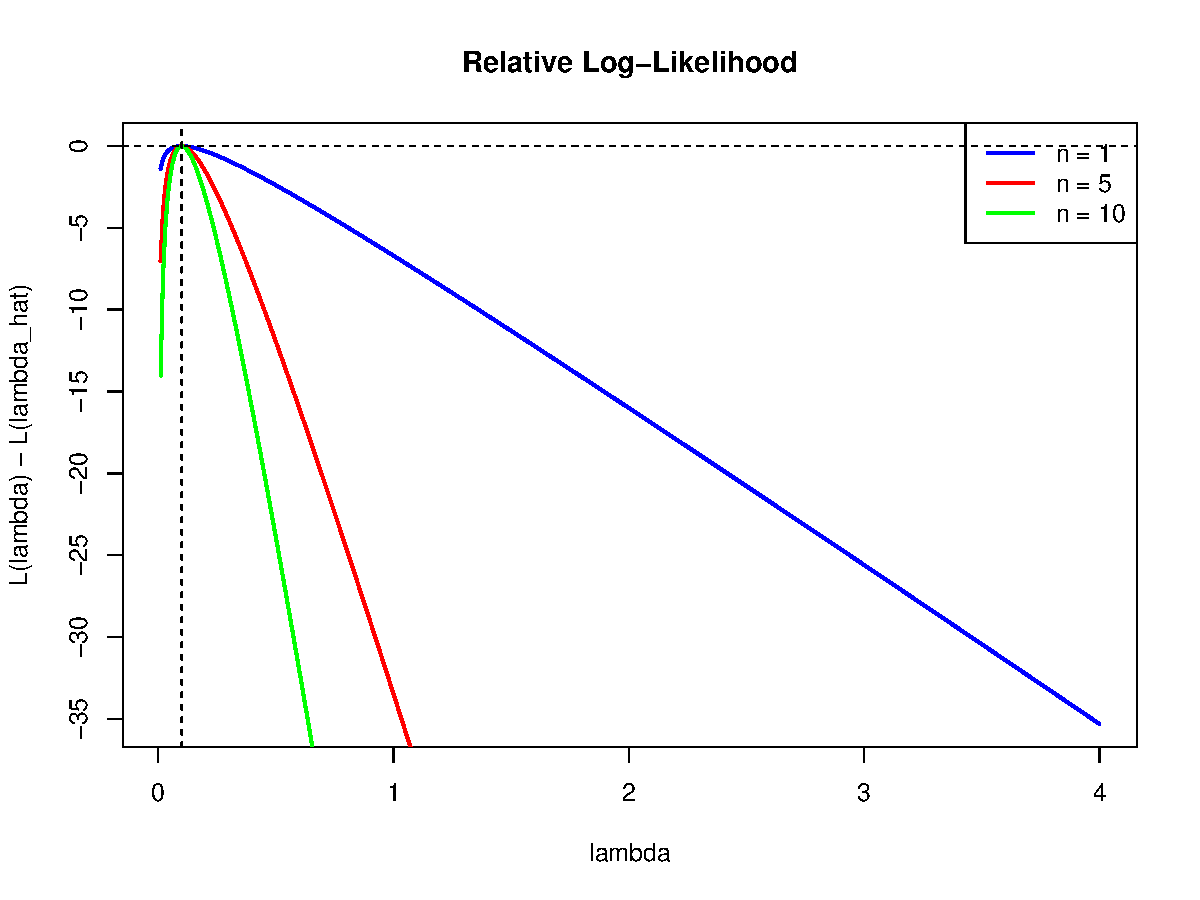
\includegraphics[width=0.8\textwidth]{Estimation_prob4_plot.pdf}
    \caption{Relative log-likelihood for the exponential MLE across different sample sizes}
\end{figure}

The vertical line is at $\hat{\lambda}=0.1$. As $n$ grows the curve becomes sharper (narrower peak), which means we are more certain about the estimate — the standard error shrinks accordingly.

\newpage
% =====================================================
% MODULE 2: CONFIDENCE INTERVALS
% =====================================================
\section{Module 2: Confidence Intervals}

\subsection{Problem 4.12: Comparing Group Means}
\textbf{Solution:}

\textbf{(a) Boxplot comparison:}
\begin{figure}[H]
    \centering
    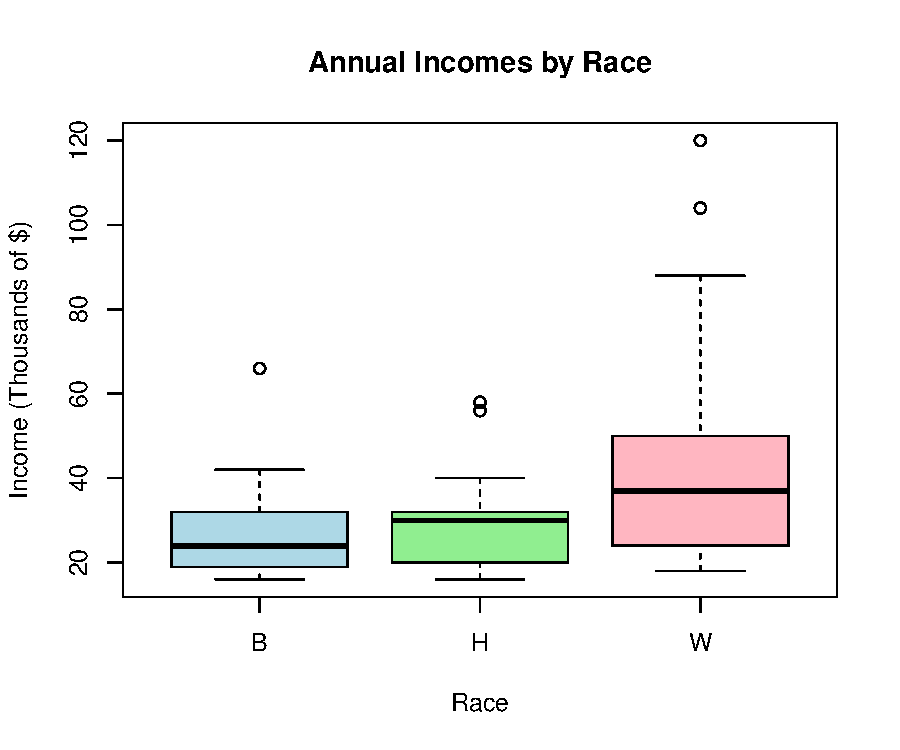
\includegraphics[width=0.7\textwidth]{CI_prob1_boxplot.pdf}
    \caption{Side-by-side boxplot of income by racial-ethnic group}
\end{figure}
The boxplot shows White households generally have higher median incomes than Hispanic and Black households. Whites also show greater spread, with more outliers at the top end.

\textbf{(b) 90\% CI assuming equal variances:}
Running \texttt{t.test(..., var.equal=TRUE, conf.level=0.90)} gives:
$$\text{90\% CI for } \mu_W - \mu_B: \quad (4.65,\ 24.81) \text{ thousand dollars}$$
Since 0 is not in this interval, there is a statistically significant income difference at the 10\% level.

\textbf{(c) 90\% CI without equal-variance assumption (Welch):}
$$\text{90\% CI}: \quad (6.94,\ 22.52) \text{ thousand dollars}$$
The Welch interval is narrower. When the two groups have quite different sample sizes, assuming equal variances inflates the standard error; Welch's correction adjusts the degrees of freedom more appropriately.

\newpage
\subsection{Problem 4.16: Comparing Proportions using Wald CI}
\textbf{Solution:}
\begin{itemize}
    \item Alcohol users: $n_1 = 1949$, marijuana users $= 955$, $\hat{p}_1 = 955/1949 = 0.490$
    \item Non-alcohol users: $n_2 = 327$, marijuana users $= 5$, $\hat{p}_2 = 5/327 = 0.0153$
\end{itemize}

\textbf{(a) Wald 95\% CI:}
$$SE(\hat{p}_1 - \hat{p}_2) = \sqrt{\frac{0.49 \times 0.51}{1949} + \frac{0.015 \times 0.985}{327}} \approx 0.01320$$
$$CI = (0.4747 - 1.96 \times 0.01320,\ 0.4747 + 1.96 \times 0.01320) = (0.4488,\ 0.5006)$$

\textbf{(b) Using \texttt{prop.test} in R:}
With \texttt{correct=FALSE}: CI = $(0.4488,\ 0.5006)$ — matches exactly.

The interval is entirely above 0, so we can say with 95\% confidence that teenagers who drink are substantially more likely to have also used marijuana. Both samples are large enough ($np > 10$) for the normal approximation to hold well here.

\subsection{Problem 4.17: Tail Behaviour of the $t$-Distribution}
\textbf{Solution:}
I simulated 10,000 observations from a $t(3)$ distribution in R.

\begin{figure}[H]
    \centering
    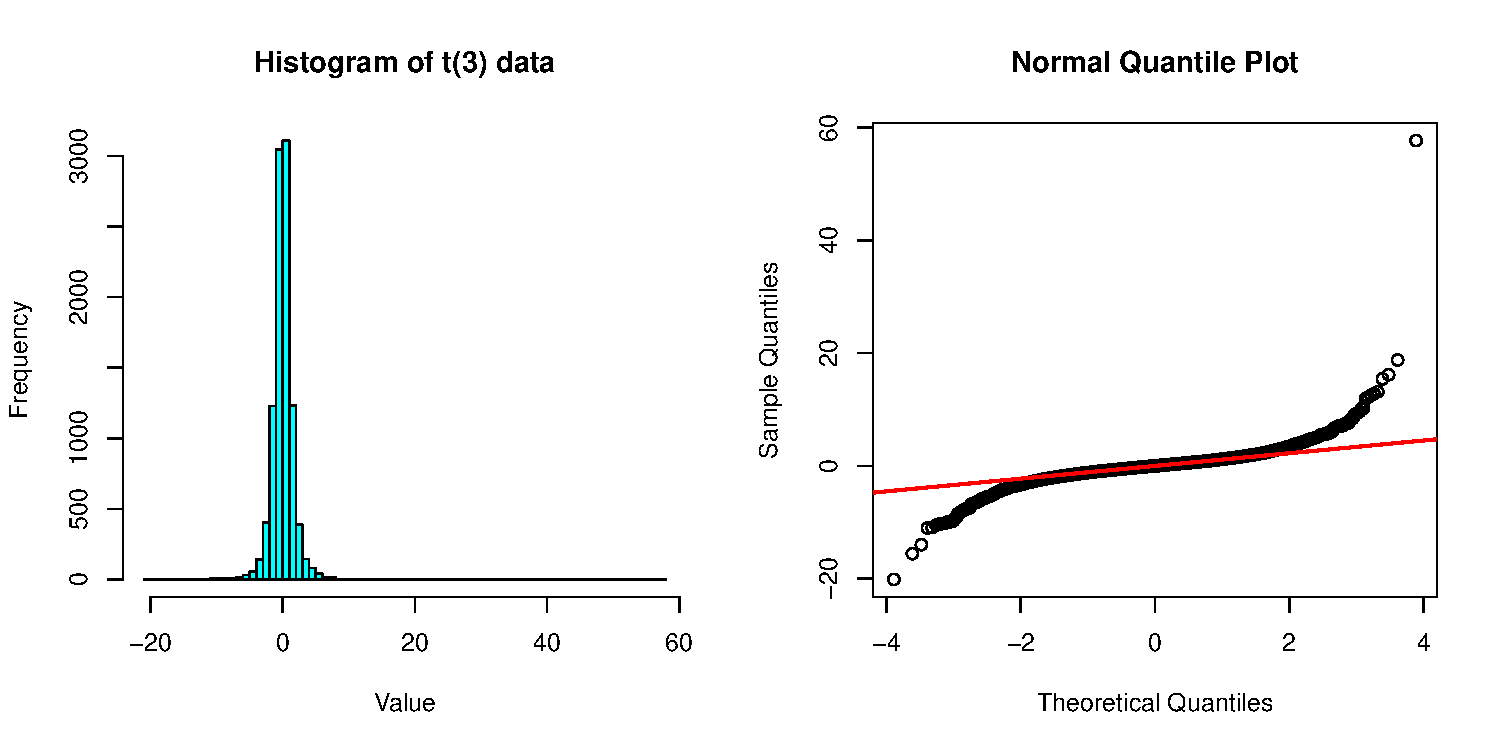
\includegraphics[width=0.9\textwidth]{CI_prob3_plots.pdf}
    \caption{Histogram and QQ-plot of $t(3)$ data}
\end{figure}

Looking at just the histogram it is hard to tell that this is not normal — it is symmetric and roughly bell-shaped. The QQ-plot is more revealing: the points curve away from the line at both ends, which is the signature of heavy tails. The $t$ with low degrees of freedom puts more probability in the extremes than the normal does, and the QQ-plot picks this up clearly.

\newpage
\subsection{Problem 4.45: Confidence Interval under Multinomial Distribution}
\textbf{Solution:}

\textbf{Part (a) -- MLE:}
With genotype probabilities $\pi^2, 2\pi(1-\pi), (1-\pi)^2$ and counts $y_1, y_2, y_3$:
$$L(\pi) = (2y_1+y_2)\ln\pi + (y_2+2y_3)\ln(1-\pi) + \text{const}$$
Setting the derivative to zero:
$$\hat{\pi} = \frac{2y_1 + y_2}{2n}$$

\textbf{Part (b) -- Fisher Information:}
$$\frac{d^2L}{d\pi^2} = -\frac{2y_1+y_2}{\pi^2} - \frac{y_2+2y_3}{(1-\pi)^2}$$
Taking expectations using $E[y_j]$ for each genotype:
$$I_n(\pi) = \frac{2n}{\pi} + \frac{2n}{1-\pi} = \frac{2n}{\pi(1-\pi)}$$
$$SE(\hat{\pi}) \approx \sqrt{\frac{\hat{\pi}(1-\hat{\pi})}{2n}}$$

\textbf{Part (c) -- 95\% Wald CI:}
For large $n$, the MLE is approximately normal, so:
$$CI_{95\%} = \hat{\pi} \pm 1.96\sqrt{\frac{\hat{\pi}(1-\hat{\pi})}{2n}}$$

\subsection{Problem 4.50: Simulation of Confidence Intervals ($p=0.06, n=20$) -- Interactive Applet}
\textbf{Solution:}

I used the applet at \url{https://istats.shinyapps.io/ExploreCoverage/} with $p=0.06$, $n=20$, and a 95\% nominal confidence level.

\textbf{(a) Wald CI, 10 samples:}
\begin{itemize}
    \item Result: 15 out of 20 intervals covered the true $p$
    \item \textbf{Coverage: 75\%}
\end{itemize}
This is well below the expected 95\%. The issue is that $n=20$ is too small for the normal approximation to work when $p$ is this close to 0 — the binomial is very skewed in this case.

\textbf{(b) Wald CI, 1000 samples:}
\begin{itemize}
    \item Result: 711 out of 1000 intervals covered the true $p$
    \item \textbf{Coverage: 71.1\%}
\end{itemize}
Even with 1000 replications, the Wald interval only achieves about 71\% coverage. The sampling distribution of $\hat{p}$ is discrete and skewed for small $n$ and small $p$ -- the normal approximation simply does not hold here.

\textbf{(c) Why Wald CI collapses when $\hat{p} = 0$:}
If all $n$ trials result in failure, then $\hat{p}=0$ and the Wald CI becomes:
$$0 \pm z\sqrt{0} = (0,0)$$
This interval has zero width and never contains a positive $p$. Since getting zero successes is quite probable when $p=0.06$ and $n=20$ (probability $\approx 0.29$), this happens often and drags the coverage way down.

\textbf{(d) Wilson Score CI, 1000 samples:}
\begin{itemize}
    \item Result: 975 out of 1000 intervals covered the true $p$
    \item \textbf{Coverage: 97.5\%}
\end{itemize}
Switching to the Wilson score interval fixes the problem. It does not collapse to a point when $\hat{p}=0$, and its coverage is close to the nominal 95\% even for small $n$ and extreme $p$.


\newpage
% =====================================================
% MODULE 3: BAYESIAN INFERENCE
% =====================================================
\section{Module 3: Bayesian Inference}

\subsection{Problem 4.64: Bias-Variance Tradeoff (Bayes vs ML Estimator)}
\textbf{Solution:}

\textbf{Part (a):}
The Bayesian estimator (using a uniform prior on $\pi$) is $\tilde{\pi} = \frac{Y+1}{n+2}$. Its bias is:
$$\text{Bias}(\tilde{\pi}) = \frac{n\pi+1}{n+2} - \pi = \frac{1-2\pi}{n+2}$$
And its variance:
$$Var(\tilde{\pi}) = \frac{n\pi(1-\pi)}{(n+2)^2}$$

Compare with the MLE $\hat{\pi} = Y/n$, which has zero bias but variance $\pi(1-\pi)/n$. The Bayes estimator is biased but its variance is smaller, especially when $n$ is small.

\textbf{Part (b): MSE comparison}
$$MSE(\tilde{\pi}) = \frac{n\pi(1-\pi)+(1-2\pi)^2}{(n+2)^2}$$

\begin{figure}[H]
    \centering
    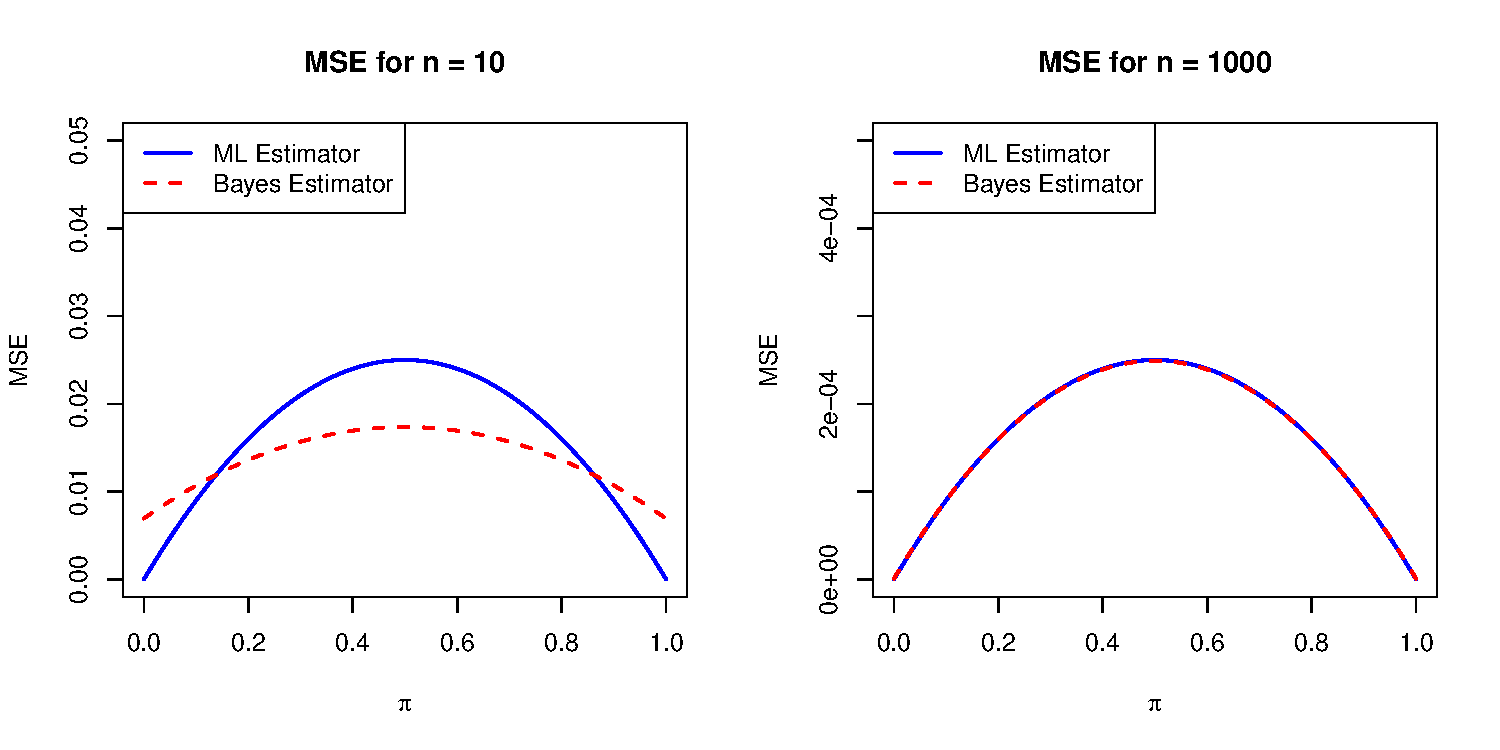
\includegraphics[width=0.9\textwidth]{Bayesian_prob1_plot.pdf}
    \caption{MSE of ML vs Bayes estimator for different values of $\pi$}
\end{figure}

For $n=10$ the Bayes MSE is lower than the ML MSE across most values of $\pi$ — the prior pulls the estimate toward 0.5, which trades a little bias for a noticeable variance reduction. By $n=1000$ the data overwhelms the prior and the two estimators behave essentially the same.

\subsection{Problem 4.66: Anorexia Study and Bayesian Shrinkage}
\textbf{Solution:}
For $\tilde{\mu} = c\bar{Y}$:
$$\text{Bias} = (c-1)\mu, \quad Var(\tilde{\mu}) = c^2 \frac{\sigma^2}{n}$$
Setting $\mu = \sigma = n = 1$:
$$MSE = (1-c)^2 + c^2 = 1 - 2c + 2c^2$$
Differentiating and setting to zero: $c_{opt} = 0.5$.

\begin{figure}[H]
    \centering
    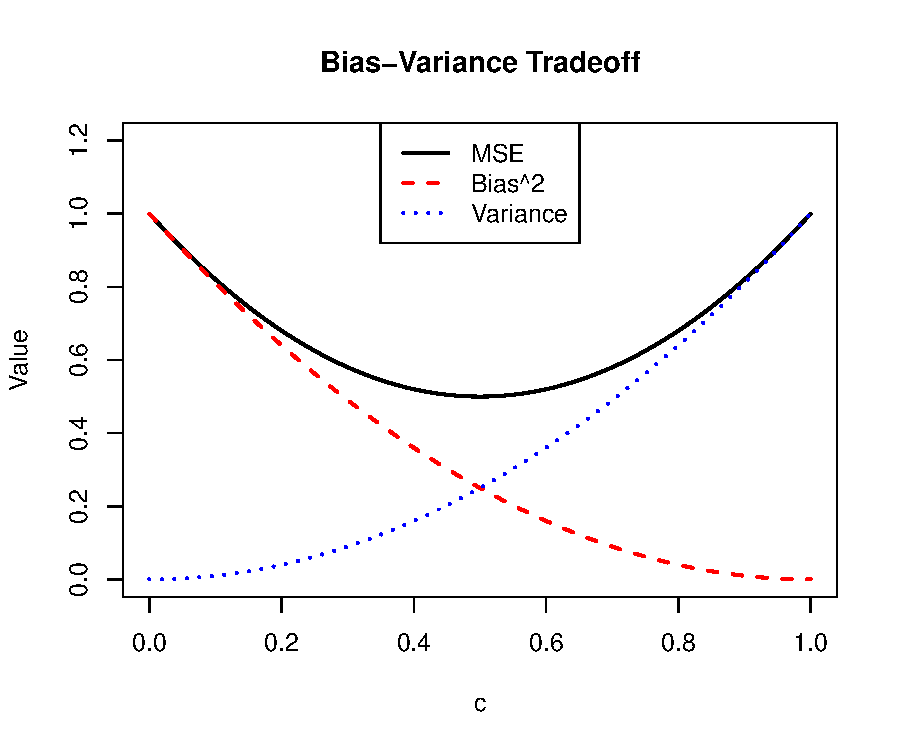
\includegraphics[width=0.55\textwidth]{Bayesian_prob2_plot.pdf}
    \caption{Bias, variance, and MSE as a function of $c$}
\end{figure}

In a Bayesian sense, multiplying $\bar{Y}$ by a constant $c < 1$ is equivalent to shrinking the estimate toward a prior mean of 0. Shrinkage always hurts a little bit in terms of bias, but when the prior is reasonable (here the true mean is small) the variance reduction more than compensates, giving a lower overall MSE. As $n$ grows, the optimal amount of shrinkage decreases — the data speak for themselves.

\newpage
\subsection{Problem 4.77: Order Statistics and Medians}
\textbf{Solution:}
The population median $M$ satisfies $P(Y_i < M) = 0.5$. If we count how many observations in a sample of size $n$ fall below $M$, that count $X$ follows $\text{Binomial}(n, 0.5)$.

We want to find indices $a$ and $b$ such that $P(Y_{(a)} \le M \le Y_{(b)}) \approx 0.95$. This is equivalent to finding $a, b$ such that $P(a \le X < b) \approx 0.95$.

For large $n$, $X \approx N(n/2,\ n/4)$, so:
$$a \approx \frac{n}{2} - 1.96 \cdot \frac{\sqrt{n}}{2}, \quad b \approx \frac{n}{2} + 1.96 \cdot \frac{\sqrt{n}}{2}$$
This gives a nonparametric 95\% CI for the median using only order statistics — no distributional assumptions needed.

\subsection{Problem 4.78: Dirichlet Conjugacy in Multinomial Models}
\textbf{Solution:}

\textbf{(a)} A uniform prior over the simplex corresponds to a $\text{Dirichlet}(\alpha_1, \dots, \alpha_c)$ with all $\alpha_j = 1$.

\textbf{(b)} The Dirichlet is conjugate to the multinomial. Combining the likelihood $L \propto \prod \pi_j^{y_j}$ with the prior $\propto \prod \pi_j^{\alpha_j-1}$ gives a posterior:
$$\pi \mid y \sim \text{Dirichlet}(y_1+\alpha_1,\ \dots,\ y_c+\alpha_c)$$

\textbf{(c)} The posterior mean for each $\pi_j$ is:
$$E[\pi_j \mid y] = \frac{y_j + \alpha_j}{n + \sum_k \alpha_k}$$
With $\alpha_j = 1$ for all $j$ (uniform prior), this becomes $\frac{y_j + 1}{n + c}$, which is exactly Laplace smoothing — adding a pseudo-count of 1 to each category before computing proportions to avoid zero estimates.

\newpage
% =====================================================
% MODULE 4: LINEAR MODELS
% =====================================================
\section{Module 4: Linear Models}

\subsection{Problem 6.1: Scottish Hill Races}
\textbf{Solution:}

\textbf{(a) Regression of men's time on women's time:}

\begin{figure}[H]
    \centering
    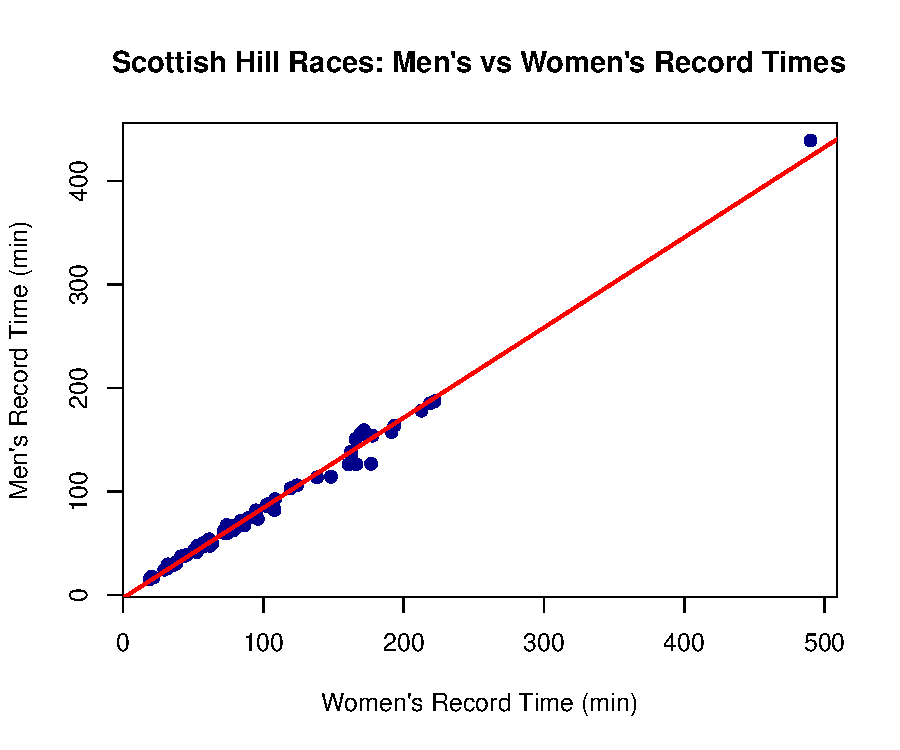
\includegraphics[width=0.45\textwidth]{Linear_prob1_scatterplot.pdf}
    \caption{Men's vs women's race times with fitted regression line}
\end{figure}

Fitted model: $\hat{\text{Time}}_M = -2.834 + 0.871 \times \text{Time}_W$

For the Highland Fling where women's time is 409.05 min, the predicted men's time is $-2.834 + 0.871 \times 409.05 \approx 353.4$ min.

\textbf{(b) Correlation:}
$r = 0.9959$. This is a very strong positive linear relationship -- as women's finishing times go up (harder/longer races), men's times increase in almost the same proportion. The two are essentially measuring the same underlying difficulty.

\textbf{(c) Regression through the origin:}
Fitting $\hat{\text{Time}}_M = \beta \times \text{Time}_W$ (no intercept) gives $\hat{\beta} = 0.8523$. So men complete the same courses in roughly 85\% of women's time. The slope is slightly higher than in (a), which makes sense once you remove the negative intercept.

\subsection{Problem 6.3: Influential Observations in Firearms Data}
\textbf{Solution:}

\begin{figure}[H]
    \centering
    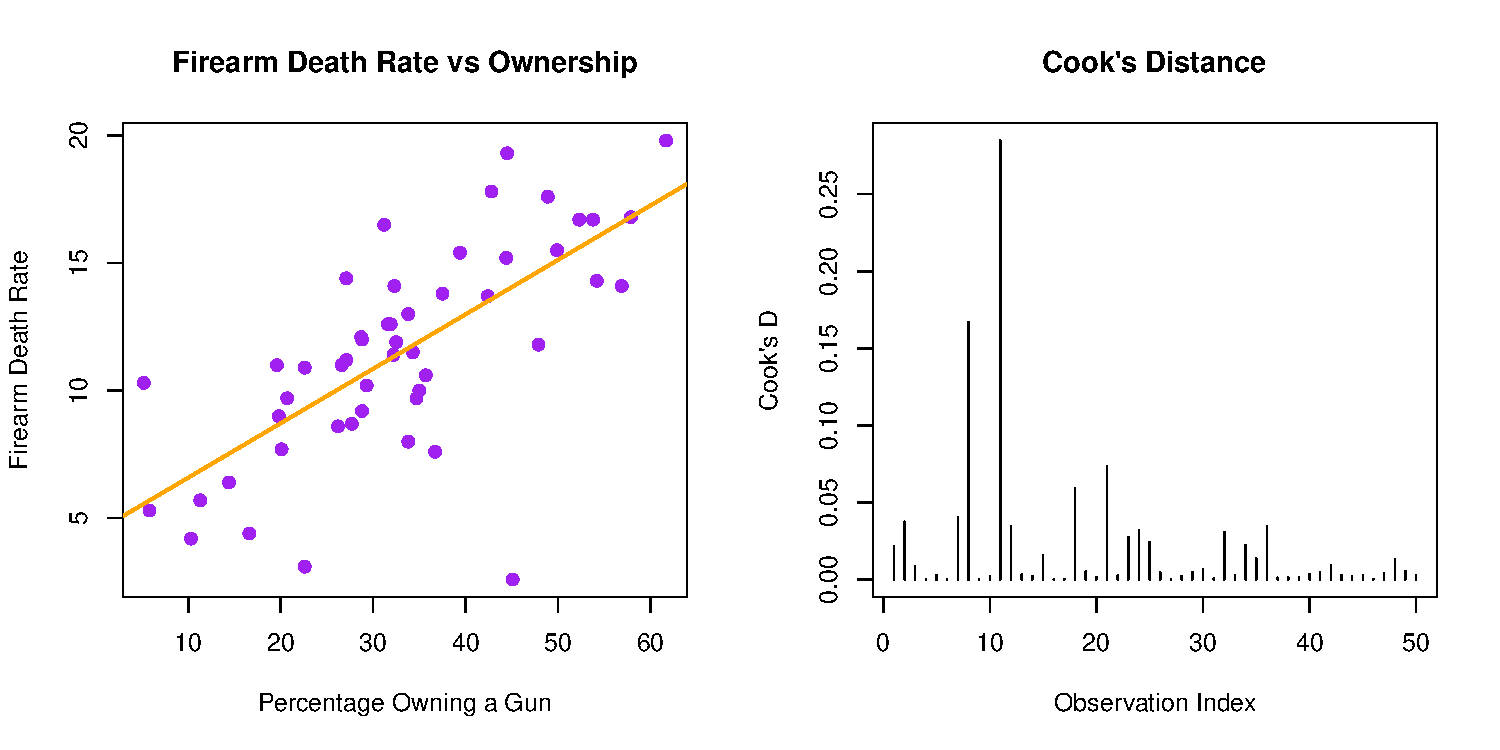
\includegraphics[width=0.8\textwidth]{Linear_prob2_plots.pdf}
    \caption{Firearms regression with Cook's distance highlighted}
\end{figure}

Computing Cook's distances, observation 11 (Hawaii) stands out with a Cook's $D \approx 0.80$, far above the next highest value of about 0.074. Hawaii has very low gun ownership and very low gun death rates, which sits far from the pattern of other states and pulls the regression line toward it.

Removing this point:
\begin{itemize}
    \item Correlation before removal: $r = 0.6976$
    \item Correlation after removal: $r = 0.7823$
\end{itemize}
The positive relationship between ownership and gun deaths becomes clearer once this outlier is removed.

\subsection{Problem 6.5: Modelling COVID-19 Case Growth}
\textbf{Solution:}

\begin{figure}[H]
    \centering
    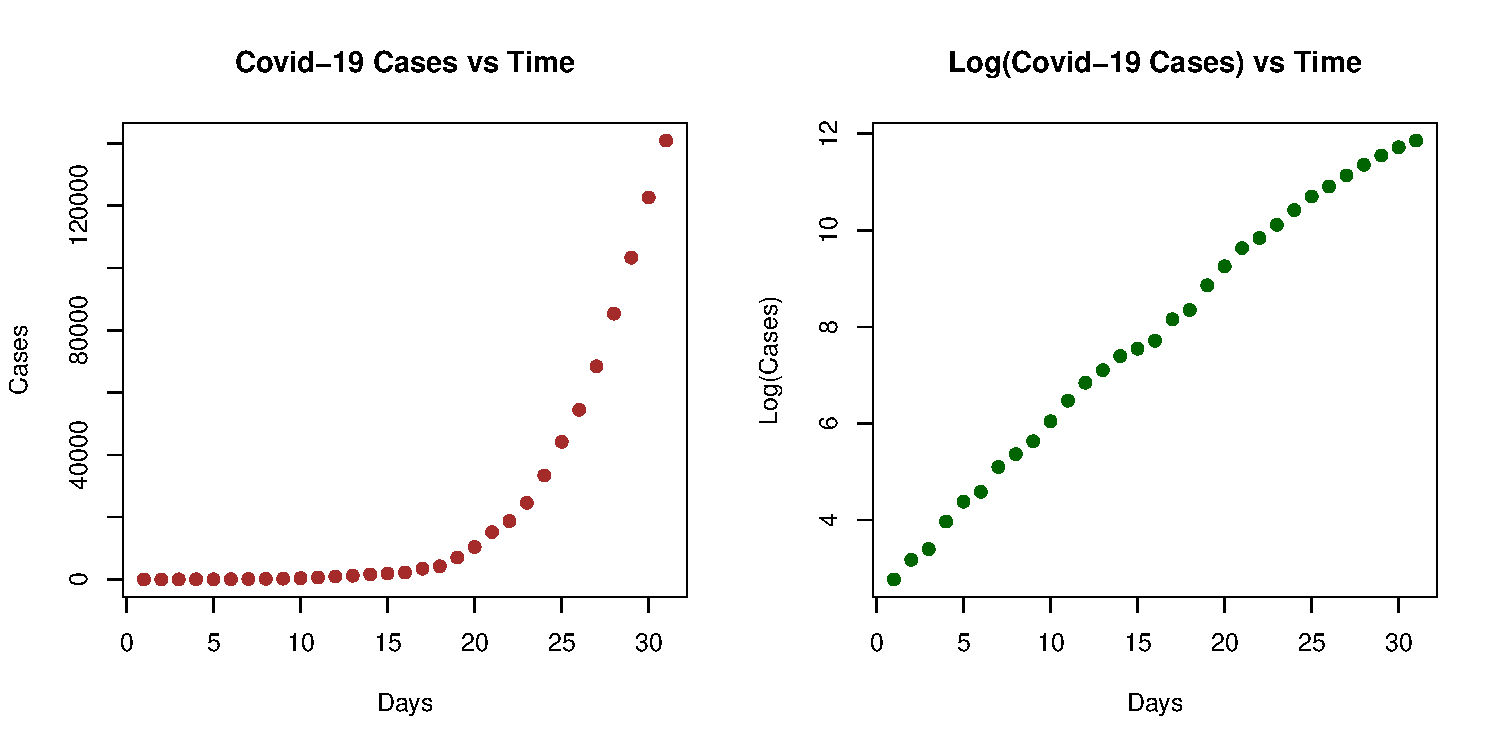
\includegraphics[width=0.85\textwidth]{Linear_prob3_scatterplots.pdf}
    \caption{Raw case counts (left) vs log-transformed (right) against days}
\end{figure}

On the raw scale, cases grow exponentially and the scatter is heavily curved. After taking logs:
\begin{itemize}
    \item Correlation with raw cases: $r \approx 0.793$
    \item Correlation with $\log(\text{cases})$: $r \approx 0.997$
\end{itemize}

The fitted log-linear model is:
$$\log(\text{cases}) = 2.843 + 0.3088 \times \text{day}$$
This means cases multiply by $e^{0.3088} \approx 1.362$ each day, i.e.\ about 36\% daily growth in the early outbreak.

\subsection{Problem 6.24: Effect of a High-Leverage Outlier}
\textbf{Solution:}
Starting with five points around a clear positive trend, the correlation is $r \approx 0.997$. When the extreme point $(15, -10)$ is added:

\begin{figure}[H]
    \centering
    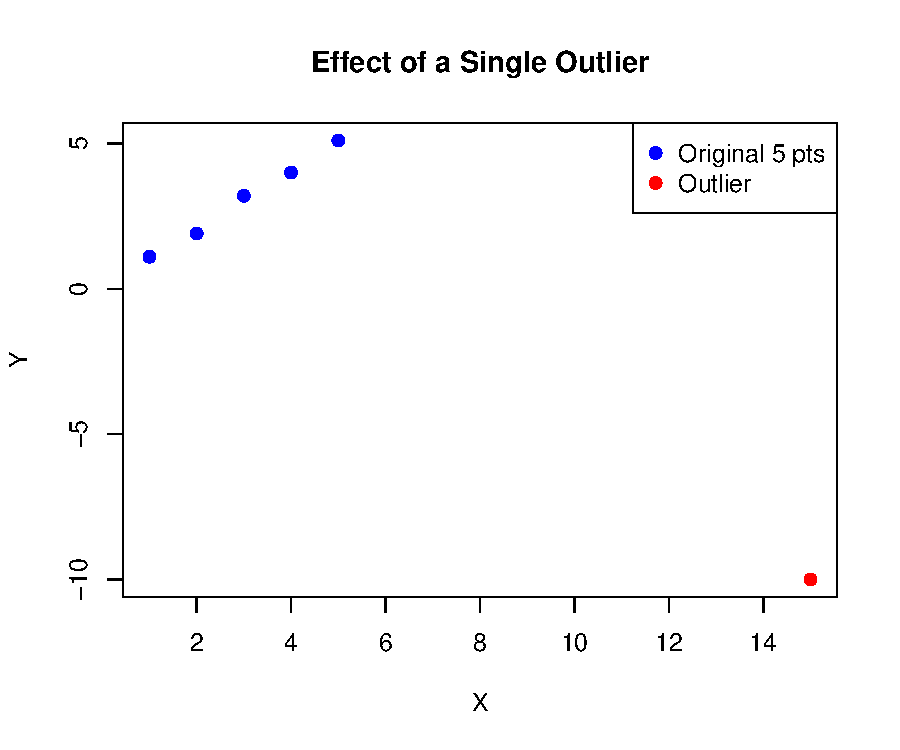
\includegraphics[width=0.45\textwidth]{Linear_prob4_outlier.pdf}
\end{figure}

The correlation flips to $r \approx -0.856$. The new point is far from the centre of the data (high leverage), and its $y$-value goes in completely the opposite direction from what the trend predicts, so it dominates the fit. Cook's distance for this point is many times larger than for any other observation, confirming it is the culprit.

\subsection{Problem 6.25: Interactive Correlation Guessing}
\textbf{Solution:}

I used the correlation guessing applet at \url{https://istats.shinyapps.io/guesscorr/}. Ten scatter plots were shown one at a time and I entered a guess for each correlation before seeing the answer.

\begin{table}[H]
\centering
\begin{tabular}{c c c}
\toprule
\textbf{Plot} & \textbf{My Guess} & \textbf{Actual} \\
\midrule
1  &  0.70  &  0.360  \\
2  & -0.05  & -0.102  \\
3  & -0.70  & -0.835  \\
4  &  0.97  &  0.992  \\
5  &  0.07  &  0.078  \\
6  &  0.12  &  0.205  \\
7  & -0.80  & -0.765  \\
8  & -0.40  & -0.383  \\
9  & -0.60  & -0.649  \\
10 &  0.06  &  0.076  \\
\bottomrule
\end{tabular}
\caption{My guesses vs the actual correlation values from the applet}
\end{table}

The correlation between my guesses and the actual values is $r = 0.9781$. Most guesses were quite close, especially for the strongly positive and negative plots (4, 3, 7). The tricky ones were the near-zero correlations like Plot 1, where I overestimated -- it is harder to visually distinguish a correlation of 0.36 from 0.6 when the cloud is fairly tight.

\subsection{Problem 6.30: Invariance of Correlation to Linear Scaling}
\textbf{Solution:}
If we replace $y$ with $y' = cy$ for some constant $c \ne 0$:
$$s_{y'} = |c| s_y, \quad \text{cov}(x, y') = c \cdot \text{cov}(x, y), \quad \hat{\beta}'_1 = c\hat{\beta}_1$$
So the correlation:
$$r' = \hat{\beta}'_1 \cdot \frac{s_x}{s_{y'}} = c\hat{\beta}_1 \cdot \frac{s_x}{|c|s_y} = \pm \hat{\beta}_1 \cdot \frac{s_x}{s_y} = \pm r$$
The sign reverses only if $c < 0$ (reflecting the axis), otherwise $r$ is completely unchanged. This is why the unit of measurement of $y$ does not matter when computing a correlation coefficient.

\end{document}
